\documentclass[11pt,letterpaper]{article}
\usepackage[margin=0.93in,headheight=15pt]{geometry}
\usepackage[T1]{fontenc}
\usepackage[utf8]{inputenc}
\usepackage{textcomp}
\usepackage{lmodern,microtype}
\usepackage{amsmath,amssymb,amsthm,mathtools}
\usepackage{booktabs,array,longtable}
\usepackage{tikz}
\usetikzlibrary{positioning,arrows.meta,calc,shapes.geometric}
\usepackage{fancyhdr}
\usepackage{xcolor}
\usepackage[colorlinks=true,linkcolor=black,citecolor=black,urlcolor=black]{hyperref}
\usepackage{enumitem}
\hypersetup{pdftitle={Certified Failure Geometry: Evidence-Cut Duality, Robust Waking, and Rare-Fault Exponents},pdfauthor={<Brian Tenneson>},pdfsubject={Finite certified evidence, destructive cuts and robustness},pdfkeywords={certified evidence, hypergraph transversals, failure cuts, robust retention, rare-fault reliability}}
\setlist[itemize]{itemsep=2pt,topsep=4pt}
\setlist[enumerate]{itemsep=3pt,topsep=4pt}
\pagestyle{fancy}
\fancyhf{}
\fancyhead[L]{\small Certified Failure Geometry}
\fancyhead[R]{\small FDWC$^3$ \quad W3}
\fancyfoot[C]{\small\thepage}
\renewcommand{\headrulewidth}{0.35pt}
\newtheorem{theorem}{Theorem}[section]
\newtheorem{lemma}[theorem]{Lemma}
\newtheorem{proposition}[theorem]{Proposition}
\newtheorem{corollary}[theorem]{Corollary}
\newtheorem{definition}[theorem]{Definition}
\newtheorem{example}[theorem]{Example}
\newtheorem{remark}[theorem]{Remark}
\newtheorem{question}[theorem]{Open question}
\DeclareMathOperator{\Min}{Min}
\DeclareMathOperator{\cost}{cost}
\DeclareMathOperator{\Anc}{Anc}
\DeclareMathOperator{\Tr}{Tr}
\DeclareMathOperator{\Core}{Core}
\DeclareMathOperator{\supp}{supp}
\newcommand{\calA}{\mathcal A}
\newcommand{\calP}{\mathcal P}
\newcommand{\calB}{\mathcal B}
\newcommand{\calH}{\mathcal H}
\newcommand{\calW}{\mathcal W}
\newcommand{\Gam}{\Gamma}
\newcommand{\wk}{\mathsf{wk}}
\newcommand{\alive}{\mathsf{alive}}
\newcommand{\fail}{\mathsf{fail}}
\newcommand{\authorname}{\textless{}Brian Tenneson\textgreater{}}
\title{\textbf{Certified Failure Geometry}\\[5pt]
\large Evidence-Cut Duality, Robust Waking, and Rare-Fault Exponents}
\author{\authorname\\
\normalsize Research conception, direction, and authorial oversight\\
\normalsize DATA MIND (OpenAI GPT-6): AI-assisted mathematical research and exposition}
\date{31 October 2026 \quad | \quad Level-3 FDWC research exposition W3}
\begin{document}
\maketitle
\vspace{-0.7em}
\begin{center}
\begin{minipage}{0.91\linewidth}
\small\noindent\textbf{AI disclaimer notice.} The complete AI-assisted authorship, reliability, and verification declaration appears on the last page. Every claim below is conditional on an explicit finite, frozen, prevalidated evidence model. No external prior-art search or independent machine proof certification has been performed, and the W0 and W1 ancestors have not been independently inspected for this W3 derivation.
\end{minipage}
\end{center}
\begin{abstract}
Retention asks which certified evidence to keep; failure geometry asks which evidence losses make a declared ability impossible. In the finite typed, validated, fixed-epoch setting of the preceding witness-selective sufficiency theory, we identify the inclusion-minimal sufficient packages with a hypergraph of positive certificates and characterize all destructive revocation sets as its minimal transversals. The duality is involutive: minimal destructive sets themselves determine the minimal sufficient packages. A packet belongs to the earlier mandatory core exactly when its individual revocation defeats joint sufficiency. We derive fault-distance and minimum fault-cost invariants, an NP-completeness result for finding a least-cost destructive set even for one query in a depth-one arena, and an exact tractable fragment when minimal witness ancestries are disjoint. A separate quantifier analysis distinguishes robust precommitted retention from post-failure adaptive selection and exhibits a sharp family of unbounded (as tolerance grows) price gaps. Under independent rare node failures, the minimum destructive weight becomes the leading failure-probability exponent, and the number of cheapest cuts becomes its leading coefficient. All results concern loss of frozen certified answers, not falsity of the answers, checker correctness, new proof discovery, or full-system experimental advantage. Originality is asserted only as a candidate development relative to the provided manuscript ancestry.
\end{abstract}
\clearpage
\tableofcontents
\clearpage
\clearpage
\section*{Reader's Glossaries: Argot and Notation}
\addcontentsline{toc}{section}{Reader's Glossaries: Argot and Notation}
\noindent\emph{Reading key.} The entries below translate the manuscript's specialized vocabulary and principal symbols into plain English. "First found" links to the opening page and section of the first substantive discussion in the body (not the earlier abstract or this glossary). The formal definitions and hypotheses in the article remain authoritative.
\subsection*{Argot: Specialized Terms}
\addcontentsline{toc}{subsection}{Argot: Specialized Terms}
\begingroup\small\setlength{\tabcolsep}{4pt}\renewcommand{\arraystretch}{1.16}
\begin{longtable}{@{}>{\raggedright\arraybackslash}p{.215\linewidth}>{\raggedright\arraybackslash}p{.585\linewidth}>{\raggedright\arraybackslash}p{.14\linewidth}@{}}
\toprule
\textbf{Entry} & \textbf{Meaning and why it matters} & \textbf{First found} \\
\midrule\endfirsthead
\multicolumn{3}{@{}l}{\footnotesize \emph{Argot: Specialized Terms (continued)}}\\
\toprule\textbf{Entry} & \textbf{Meaning and why it matters} & \textbf{First found} \\
\midrule\endhead
\bottomrule\endfoot
\textbf{Frozen evidence arena} & Fixed validated packets and dependencies; the analysis does not predict new proof discovery. & \hyperref[gl-first-W3-s2]{\S\,\ref*{gl-first-W3-s2}, p.\,\pageref*{gl-first-W3-s2}} \\
\textbf{Conditional invalidation} & A declared packet failure makes it and its dependents unavailable, leaving other validity unchanged. & \hyperref[gl-first-W3-s2]{\S\,\ref*{gl-first-W3-s2}, p.\,\pageref*{gl-first-W3-s2}} \\
\textbf{Positive certificate} & An inclusion-minimal dependency-complete package sufficient for required answers. & \hyperref[gl-first-W3-s2]{\S\,\ref*{gl-first-W3-s2}, p.\,\pageref*{gl-first-W3-s2}} \\
\textbf{Destructive cut} & An inclusion-minimal set of packet invalidations that leaves the required answers unwarranted. & \hyperref[gl-first-W3-s3]{\S\,\ref*{gl-first-W3-s3}, p.\,\pageref*{gl-first-W3-s3}} \\
\textbf{Transversal / hitting set} & A set meeting every positive certificate, thereby defeating all possible sufficient packages. & \hyperref[gl-first-W3-s3]{\S\,\ref*{gl-first-W3-s3}, p.\,\pageref*{gl-first-W3-s3}} \\
\textbf{Positive-negative duality} & Survival occurs precisely when at least one positive certificate avoids the failed packets. & \hyperref[gl-first-W3-s3]{\S\,\ref*{gl-first-W3-s3}, p.\,\pageref*{gl-first-W3-s3}} \\
\textbf{Involution} & The minimal positive packages can be recovered exactly from the minimal destructive cuts. & \hyperref[gl-first-W3-s3]{\S\,\ref*{gl-first-W3-s3}, p.\,\pageref*{gl-first-W3-s3}} \\
\textbf{Mandatory core} & Packets found in every sufficient package; each is a single point of failure if revoked. & \hyperref[gl-first-W3-s3]{\S\,\ref*{gl-first-W3-s3}, p.\,\pageref*{gl-first-W3-s3}} \\
\textbf{Shared-prerequisite vulnerability} & Two alternative warrants may fail together when they rely on one common ancestor. & \hyperref[gl-first-W3-s3]{\S\,\ref*{gl-first-W3-s3}, p.\,\pageref*{gl-first-W3-s3}} \\
\textbf{Global survival} & At least one valid package remains in the entire surviving arena, even if a previous choice fails. & \hyperref[gl-first-W3-s2]{\S\,\ref*{gl-first-W3-s2}, p.\,\pageref*{gl-first-W3-s2}} \\
\textbf{Fault distance} & Smallest number of directly invalidated packet identities needed to destroy sufficiency. & \hyperref[gl-first-W3-s4]{\S\,\ref*{gl-first-W3-s4}, p.\,\pageref*{gl-first-W3-s4}} \\
\textbf{Destructive weight} & Smallest total assigned fault weight of a set that destroys sufficiency. & \hyperref[gl-first-W3-s4]{\S\,\ref*{gl-first-W3-s4}, p.\,\pageref*{gl-first-W3-s4}} \\
\textbf{Disjoint-ancestry fragment} & Special case with nonoverlapping minimal witness supports, allowing an easier exact computation. & \hyperref[gl-first-W3-s4]{\S\,\ref*{gl-first-W3-s4}, p.\,\pageref*{gl-first-W3-s4}} \\
\textbf{Robust commitment} & Select one retention package in advance that must survive every allowed fault pattern. & \hyperref[gl-first-W3-s5]{\S\,\ref*{gl-first-W3-s5}, p.\,\pageref*{gl-first-W3-s5}} \\
\textbf{Adaptive retention} & Choose a possibly different surviving package after learning which fault occurred. & \hyperref[gl-first-W3-s5]{\S\,\ref*{gl-first-W3-s5}, p.\,\pageref*{gl-first-W3-s5}} \\
\textbf{Commitment-adaptation gap} & Extra declared retention charge caused by selecting evidence before faults are known. & \hyperref[gl-first-W3-s5]{\S\,\ref*{gl-first-W3-s5}, p.\,\pageref*{gl-first-W3-s5}} \\
\textbf{Rare-fault exponent} & Leading power of a small failure parameter in the modeled probability of losing sufficiency. & \hyperref[gl-first-W3-s6]{\S\,\ref*{gl-first-W3-s6}, p.\,\pageref*{gl-first-W3-s6}} \\
\textbf{Leading coefficient} & Number of cheapest-weight destructive cuts contributing to the leading failure term. & \hyperref[gl-first-W3-s6]{\S\,\ref*{gl-first-W3-s6}, p.\,\pageref*{gl-first-W3-s6}} \\
\end{longtable}\endgroup
\subsection*{Notation: Symbols and Abbreviations}
\addcontentsline{toc}{subsection}{Notation: Symbols and Abbreviations}
\begingroup\small\setlength{\tabcolsep}{4pt}\renewcommand{\arraystretch}{1.16}
\begin{longtable}{@{}>{\raggedright\arraybackslash}p{.215\linewidth}>{\raggedright\arraybackslash}p{.585\linewidth}>{\raggedright\arraybackslash}p{.14\linewidth}@{}}
\toprule
\textbf{Entry} & \textbf{Meaning and why it matters} & \textbf{First found} \\
\midrule\endfirsthead
\multicolumn{3}{@{}l}{\footnotesize \emph{Notation: Symbols and Abbreviations (continued)}}\\
\toprule\textbf{Entry} & \textbf{Meaning and why it matters} & \textbf{First found} \\
\midrule\endhead
\bottomrule\endfoot
\textbf{$A$} & The finite set of validated, currently authorized packet identities. & \hyperref[gl-first-W3-s2]{\S\,\ref*{gl-first-W3-s2}, p.\,\pageref*{gl-first-W3-s2}} \\
\textbf{$p\preceq v$} & Packet $p$ is a prerequisite ancestor of packet $v$. & \hyperref[gl-first-W3-s2]{\S\,\ref*{gl-first-W3-s2}, p.\,\pageref*{gl-first-W3-s2}} \\
\textbf{$\downarrow v$} & A warrant packet and all of its prerequisite packets. & \hyperref[gl-first-W3-s2]{\S\,\ref*{gl-first-W3-s2}, p.\,\pageref*{gl-first-W3-s2}} \\
\textbf{$\operatorname{Anc}(Q)$} & Union of the prerequisite closures of all packets in $Q$. & \hyperref[gl-first-W3-s2]{\S\,\ref*{gl-first-W3-s2}, p.\,\pageref*{gl-first-W3-s2}} \\
\textbf{$S_L$} & Queries already warranted by the stable live evidence base. & \hyperref[gl-first-W3-s2]{\S\,\ref*{gl-first-W3-s2}, p.\,\pageref*{gl-first-W3-s2}} \\
\textbf{$W_\gamma$} & Alternative certified warrants available for specific query $\gamma$. & \hyperref[gl-first-W3-s2]{\S\,\ref*{gl-first-W3-s2}, p.\,\pageref*{gl-first-W3-s2}} \\
\textbf{$\Gamma$} & Required finite collection of query obligations. & \hyperref[gl-first-W3-s2]{\S\,\ref*{gl-first-W3-s2}, p.\,\pageref*{gl-first-W3-s2}} \\
\textbf{$R,\uparrow R$} & Directly invalidated packet set and all its dependent descendants. & \hyperref[gl-first-W3-s2]{\S\,\ref*{gl-first-W3-s2}, p.\,\pageref*{gl-first-W3-s2}} \\
\textbf{$A_R$} & Surviving valid arena after removing the invalidated packets and descendants. & \hyperref[gl-first-W3-s2]{\S\,\ref*{gl-first-W3-s2}, p.\,\pageref*{gl-first-W3-s2}} \\
\textbf{$\mathcal F_\Gamma$} & All dependency-complete evidence packages sufficient for $\Gamma$. & \hyperref[gl-first-W3-s2]{\S\,\ref*{gl-first-W3-s2}, p.\,\pageref*{gl-first-W3-s2}} \\
\textbf{$\mathcal P_\Gamma$} & Inclusion-minimal sufficient packages (positive certificates). & \hyperref[gl-first-W3-s2]{\S\,\ref*{gl-first-W3-s2}, p.\,\pageref*{gl-first-W3-s2}} \\
\textbf{$\operatorname{Tr}(\mathcal H)$} & Inclusion-minimal hitting sets for family $\mathcal H$. & \hyperref[gl-first-W3-s3]{\S\,\ref*{gl-first-W3-s3}, p.\,\pageref*{gl-first-W3-s3}} \\
\textbf{$\mathcal B_\Gamma$} & Inclusion-minimal destructive cuts, equal to $\operatorname{Tr}(\mathcal P_\Gamma)$. & \hyperref[gl-first-W3-s3]{\S\,\ref*{gl-first-W3-s3}, p.\,\pageref*{gl-first-W3-s3}} \\
\textbf{$\operatorname{Core}(\Gamma)$} & Intersection of all sufficient packages; matches singleton destructive cuts. & \hyperref[gl-first-W3-s3]{\S\,\ref*{gl-first-W3-s3}, p.\,\pageref*{gl-first-W3-s3}} \\
\textbf{$r(v),r(R)$} & Positive integer fault weight per packet and sum over a failed set. & \hyperref[gl-first-W3-s4]{\S\,\ref*{gl-first-W3-s4}, p.\,\pageref*{gl-first-W3-s4}} \\
\textbf{$d(\Gamma)$} & Minimum cardinality of a destructive cut. & \hyperref[gl-first-W3-s4]{\S\,\ref*{gl-first-W3-s4}, p.\,\pageref*{gl-first-W3-s4}} \\
\textbf{$\lambda_r(\Gamma)$} & Smallest total weight among destructive cuts. & \hyperref[gl-first-W3-s4]{\S\,\ref*{gl-first-W3-s4}, p.\,\pageref*{gl-first-W3-s4}} \\
\textbf{$\rho_k(\Gamma)$} & Minimum cost of one advance-committed package surviving all sets of at most $k$ faults. & \hyperref[gl-first-W3-s5]{\S\,\ref*{gl-first-W3-s5}, p.\,\pageref*{gl-first-W3-s5}} \\
\textbf{$\alpha_k(\Gamma)$} & Worst-case minimum package cost when selection is allowed after seeing a fault. & \hyperref[gl-first-W3-s5]{\S\,\ref*{gl-first-W3-s5}, p.\,\pageref*{gl-first-W3-s5}} \\
\textbf{$t,\Pr_t(\mathsf{Loss}_\Gamma)$} & Small rare-fault parameter and modeled probability of losing required answers. & \hyperref[gl-first-W3-s6]{\S\,\ref*{gl-first-W3-s6}, p.\,\pageref*{gl-first-W3-s6}} \\
\textbf{$N_r(\Gamma)$} & Number of destructive cuts having the minimum fault weight. & \hyperref[gl-first-W3-s6]{\S\,\ref*{gl-first-W3-s6}, p.\,\pageref*{gl-first-W3-s6}} \\
\end{longtable}\endgroup
\clearpage

\section{From retention to destruction}\label{gl-first-W3-s1}
The immediate predecessor W2, \emph{Certified Wake Sufficiency and Evidence Frontiers} \cite{W2}, studies a frozen set of already validated alternative warrants. Its primary task is to choose a dependency-complete package that answers named post-wake questions for the least declared retention charge. The reported W0 singleton-ATP design supplies role-attributed victories, typed validation, and wake authorization \cite{W0}; the reported W1 multiarticle supplies exact packet ancestry and fixed-witness closure \cite{W1}. W2's key innovation relative to that reported ancestry is to allow alternative checked witnesses for one question.

This article changes the question. Suppose the entire finite pool was correctly validated at the start of the epoch. Some packet identities are subsequently invalidated, along with everything dependent on them. \emph{Which patterns of invalidation destroy the ability to answer a specified collection of questions?} Can those patterns be recovered from the sufficient packages alone? What is the precise price of ensuring that an answer survives several faults, and how does worst-case resilience control the probability of failure when faults are rare?

The mathematical object that emerges is a \emph{pair of dual antichains}: minimal positive packages and minimal destructive cuts. This is a specialization of elementary finite-set duality to typed, dependency-closed mathematical evidence. The formulation is not a priority claim for hypergraph transversal theory or reliability asymptotics in general. Its contribution relative to W2 is a different invariant and the consequences proved below.

\paragraph{Interpretation.} To ``destroy a query'' means to destroy \emph{its warranted availability in the stipulated finite arena}. It never means to refute the underlying mathematical statement. The only packets capable of warranting a query are the prevalidated, appropriately typed and authorized alternatives explicitly listed at the frozen epoch. Nothing in this model generates a new proof or authorizes a previously invalid projection.

\section{Finite evidence model and survivor packages}\label{gl-first-W3-s2}
\begin{definition}[Frozen certified evidence arena]\label{def:arena}
Let $A$ be a finite set of packet identities with a directed acyclic prerequisite graph. If a packet $p$ is a prerequisite of $v$, write $p\preceq v$, allowing equality, and set
\[
\downarrow v=\{p\in A:p\preceq v\},\qquad
\Anc(Q)=\bigcup_{v\in Q}\downarrow v.
\]
An \emph{ideal} $J\subseteq A$ is a downward-closed subset. There is a fixed finite query pool $U$, a subset $S_L$ already warranted by a stable live base, and for each $\gamma\in U\setminus S_L$ an explicitly listed set $W_\gamma\subseteq A$ of separately validated, version-matched, type-correct, scope-authorized alternative warrant packets. For the remainder of the article, $\Gam\subseteq U\setminus S_L$ is \emph{finite, nonempty, and feasible}: every $W_\gamma$ for $\gamma\in\Gam$ is nonempty.

For an ideal $J$, its frozen warrant map is
\[
S(J)=S_L\cup\{\gamma\in U\setminus S_L:J\cap W_\gamma\ne\varnothing\}.
\]
Every ideal is admissible, adding retained evidence never removes validity, and exact internal dependencies have all been recorded. All external prerequisites are already valid in the stable live base. The additive incremental retention charge $c:A\to\mathbb Q_{\ge0}$ is fixed, with $\cost(J)=\sum_{v\in J}c(v)$. Costs do not include proof discovery or checking.
\end{definition}

\begin{definition}[Conditional invalidation and surviving support]\label{def:invalidate}
For a set of newly invalidated packet identities $R\subseteq A$, define
\[
\uparrow R=\{v\in A:\exists r\in R\ (r\preceq v)\},\qquad
A_R=A\setminus\uparrow R.
\]
We assume that every packet outside $\uparrow R$ retains its prior validity, version, scope, permissions and exact meaning, and that $S_L$ is unchanged. The surviving portion of a committed ideal $J$ is $J_R=J\cap A_R$. We say $\Gam$ \emph{survives in $J$ after $R$} if $\Gam\subseteq S(J_R)$; \emph{global survival} means $\Gam\subseteq S(A_R)$.
\end{definition}

This is W2's conditional, fixed-version revocation discipline, made an explicit variable of study. It is not a model of arbitrary changes of the checker, negative admission tests, or authorization policy.

\begin{definition}[Minimal positive certificates]\label{def:positive}
Put
\[
\mathcal F_\Gam=\{J\subseteq A:J\text{ is an ideal and }\Gam\subseteq S(J)\},
\qquad
\calP_\Gam=\Min_{\subseteq}\mathcal F_\Gam.
\]
Here $\Min_{\subseteq}$ removes every member strictly containing another member of the same finite family. The nonempty finite family $\calP_\Gam$ is the \emph{positive-package clutter}: its members are incomparable and nonempty.
\end{definition}

\begin{lemma}[Positive certificate representation]\label{lem:normal}
\[
\calP_\Gam
=\Min_{\subseteq}\left\{
\bigcup_{\gamma\in\Gam}\downarrow w_\gamma:
(w_\gamma)_{\gamma\in\Gam}\in\prod_{\gamma\in\Gam}W_\gamma
\right\}.
\tag{1}\label{eq:positive}
\]
Moreover, a subset $J\subseteq A$ is an ideal sufficient for $\Gam$ if and only if it contains some $P\in\calP_\Gam$.
\end{lemma}
\begin{proof}
If an ideal $J$ is sufficient, choose $w_\gamma\in J\cap W_\gamma$ for each required query. Downward closure forces $\bigcup_\gamma\downarrow w_\gamma\subseteq J$. That union is itself a sufficient ideal. Finiteness allows descent to an inclusion-minimal sufficient ideal; conversely every displayed union is sufficient. Therefore the minimal members of the two families agree. Any sufficient ideal contains a minimal sufficient subideal, while an ideal containing one is sufficient by monotonicity.
\end{proof}
\begin{remark}
Lemma \ref{lem:normal} restates the substance of W2's witness-selection normal form, with all antecedent credit retained \cite{W2}. It is the starting tool, \emph{not} a W3 originality claim. The nonempty assumption on $\Gam$ is only to avoid a degenerate empty certificate in the transversal results.
\end{remark}

\section{The duality between surviving evidence and destructive cuts}\label{gl-first-W3-s3}
\begin{lemma}[No hidden descendant fault]\label{lem:idealavoid}
For every ideal $P\subseteq A$ and every $R\subseteq A$,
\[
P\subseteq A_R\quad\Longleftrightarrow\quad P\cap R=\varnothing.
\tag{2}\label{eq:avoid}
\]
\end{lemma}
\begin{proof}
If $P\subseteq A_R$, it certainly misses $R\subseteq\uparrow R$. Conversely, if $v\in P\cap\uparrow R$, some $r\in R$ satisfies $r\preceq v$. Since $P$ is downward closed, $r\in P$, contradicting $P\cap R=\varnothing$.
\end{proof}

\begin{definition}[Transversal and cut clutter]\label{def:transversal}
For any nonempty family $\mathcal H$ of nonempty subsets of $A$, a set $R\subseteq A$ \emph{hits} $\mathcal H$ when $R\cap H\ne\varnothing$ for every $H\in\mathcal H$. Write
\[
\Tr(\mathcal H)=\Min_{\subseteq}\{R\subseteq A:\forall H\in\mathcal H,\ R\cap H\ne\varnothing\}.
\]
Define the \emph{minimal certified failure cuts} of $\Gam$ by $\calB_\Gam=\Tr(\calP_\Gam)$.
\end{definition}

\begin{theorem}[Exact positive--negative certificate duality]\label{thm:duality}
For any revocation set $R\subseteq A$, the following statements are equivalent:
\begin{enumerate}[label=(\roman*)]
\item $\Gam$ survives globally in the conditional surviving arena $A_R$;
\item some inclusion-minimal positive package $P\in\calP_\Gam$ avoids $R$;
\item $R$ does not hit every member of $\calP_\Gam$;
\item no cut $B\in\calB_\Gam$ is contained in $R$.
\end{enumerate}
Consequently, $R$ destroys joint sufficiency exactly when it contains a minimal destructive cut. The loss map is monotone in $R$.
\end{theorem}
\begin{proof}
The surviving arena $A_R$ is an ideal: every prerequisite of a packet without revoked ancestors is also without revoked ancestors. Global survival is therefore equivalent, by Lemma \ref{lem:normal}, to the existence of $P\in\calP_\Gam$ with $P\subseteq A_R$. Lemma \ref{lem:idealavoid} turns this into $P\cap R=\varnothing$, proving (i)--(iii). If $R$ hits every member of $\calP_\Gam$, finiteness supplies a minimal hitting subset $B\subseteq R$, and $B\in\calB_\Gam$. Conversely any such $B$ forces $R$ to hit every $P$. Enlargement of a hitting set cannot restore a missed package.
\end{proof}

\begin{corollary}[Direct single-query cut representation]\label{cor:singlecuts}
For each non-live query $\gamma$ with a nonempty validated warrant list,
\[
\calB_{\{\gamma\}}=
\Tr\bigl(\{\downarrow w:w\in W_\gamma\}\bigr)
=\Tr\bigl(\Min_{\subseteq}\{\downarrow w:w\in W_\gamma\}\bigr).
\tag{3a}\label{eq:singlecuts}
\]
In particular, the destructive sets are transversals of \emph{whole dependency closures}, not cuts of ordinary directed-path reachability.
\end{corollary}
\begin{proof}
The warrant $w$ survives exactly when $R\cap\downarrow w=\varnothing$. Thus the query fails precisely when $R$ meets every listed ancestry. Removing an ancestry that strictly contains another does not change the hitting condition; taking inclusion-minimal hitting sets gives both equalities.
\end{proof}

\begin{theorem}[Involution of finite evidence cuts]\label{thm:involution}
For the positive-package clutter of any feasible nonempty $\Gam$,
\[
\Tr\bigl(\calB_\Gam\bigr)=\calP_\Gam.
\tag{3}\label{eq:involution}
\]
Thus the family of minimal failure patterns uniquely determines the family of minimal positive packages, and vice versa.
\end{theorem}
\begin{proof}
We prove a finite-set statement that does not require the graph. Let $\mathcal H$ be any nonempty antichain of nonempty subsets of $A$. A set $X\subseteq A$ hits every member of $\Tr(\mathcal H)$ if and only if $X$ contains at least one $H\in\mathcal H$.

For the forward implication, suppose no $H$ is contained in $X$. Then each $H$ meets $A\setminus X$. Therefore $A\setminus X$ is a hitting set of $\mathcal H$ and contains a minimal hitting set $B\in\Tr(\mathcal H)$, disjoint from $X$: contradiction. Conversely, if $H\subseteq X$ for some $H\in\mathcal H$, every transversal $B$ of $\mathcal H$ meets $H$ and hence meets $X$. The inclusion-minimal sets $X$ containing an $H$ are precisely the members of $\mathcal H$, by its antichain property. Apply this statement with $\mathcal H=\calP_\Gam$.
\end{proof}

\begin{corollary}[The old compulsory core is exactly the single-point fault set]\label{cor:core}
Let $\Core(\Gam)=\bigcap_{J\in\mathcal F_\Gam}J$, as in W2. For every $p\in A$,
\[
p\in\Core(\Gam)\quad\Longleftrightarrow\quad \{p\}\in\calB_\Gam.
\tag{4}\label{eq:core}
\]
In particular, $\Core(\Gam)=\varnothing$ if and only if \emph{every single packet invalidation} preserves the global attainability of $\Gam$.
\end{corollary}
\begin{proof}
Every sufficient ideal contains a member of $\calP_\Gam$, so the intersection of all sufficient ideals equals $\bigcap_{P\in\calP_\Gam}P$. Thus $p$ belongs to the core exactly when $\{p\}$ hits every $P$. Since all $P$ are nonempty, the empty set hits none of them; consequently such a singleton is inclusion-minimal among hitting sets. The last assertion applies Theorem \ref{thm:duality} to every singleton.
\end{proof}

\begin{example}[Two warrants are not necessarily two protections]\label{ex:shared}
Consider a single required query $\gamma$ with two alternative checked warrants $a,b$. If $a,b$ have no prerequisites, then $\calP_{\{\gamma\}}=\{\{a\},\{b\}\}$ and $\calB_{\{\gamma\}}=\{\{a,b\}\}$. Both warrants must be invalidated to lose the query.

Now add a packet $s$ which is a shared prerequisite of both warrants. The positive packages become $\{s,a\}$ and $\{s,b\}$. The minimal cuts are $\{s\}$ and $\{a,b\}$. One failed shared prerequisite now destroys the answer even when neither of the two warrant packets has been individually invalidated.
\end{example}

\begin{remark}[Selected-package loss versus global failure]\label{rem:relative}
A cut in $\calB_\Gam$ destroys the answer in the \emph{full prevalidated arena}, even after the system is allowed to select a different surviving package. The fault set that defeats a specific precommitted $J$ can be smaller. For two independent alternative witnesses $a,b$, the committed package $J=\{a\}$ loses its answer upon revoking $a$, whereas the full arena survives that fault by switching to $b$. Its sole global minimal cut is $\{a,b\}$. This difference is why committed retention and post-fault selection require different quantifier orders in Section~\ref{sec:commit}.
\end{remark}

\begin{figure}[ht]
\centering
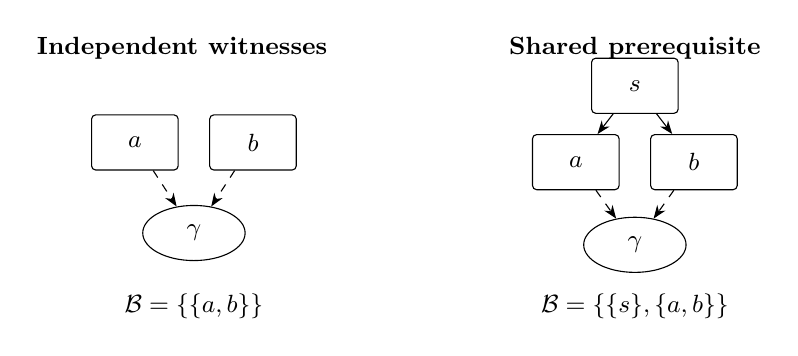
\begin{tikzpicture}[>=Stealth,every node/.style={font=\small},packet/.style={draw,rounded corners=1.5pt,minimum width=11mm,minimum height=7mm},query/.style={draw,ellipse,minimum width=13mm,minimum height=7mm}]
\node at (0.6,2.1) {\textbf{Independent witnesses}};
\node[packet] (a) at (0,0.9) {$a$}; \node[packet] (b) at (1.5,0.9) {$b$};
\node[query] (q) at (0.75,-0.25) {$\gamma$};
\draw[dashed,-{Stealth}] (a) -- (q); \draw[dashed,-{Stealth}] (b) -- (q);
\node[align=center] at (0.75,-1.18) {$\calB=\{\{a,b\}\}$};
\node at (6.35,2.1) {\textbf{Shared prerequisite}};
\node[packet] (s) at (6.35,1.62) {$s$};
\node[packet] (aa) at (5.6,0.65) {$a$}; \node[packet] (bb) at (7.1,0.65) {$b$};
\node[query] (qq) at (6.35,-0.4) {$\gamma$};
\draw[-{Stealth}] (s)--(aa);\draw[-{Stealth}] (s)--(bb);
\draw[dashed,-{Stealth}] (aa)--(qq);\draw[dashed,-{Stealth}] (bb)--(qq);
\node at (6.35,-1.18) {$\calB=\{\{s\},\{a,b\}\}$};
\end{tikzpicture}
\caption{Solid arrows are exact evidence prerequisites; dashed arrows are independently checked query-warrant projections. The right architecture has a one-node destructive cut absent on the left. Neither diagram authorizes a cross-type bridge.}
\label{fig:cuts}
\end{figure}

\begin{proposition}[Failure of joint sufficiency is a union of individual failures]\label{prop:queryunion}
Writing $\calB_\gamma=\calB_{\{\gamma\}}$ for $\gamma\in\Gam$,
\[
\calB_\Gam=\Min_{\subseteq}\left(\bigcup_{\gamma\in\Gam}\calB_\gamma\right).
\tag{5}\label{eq:unioncuts}
\]
\end{proposition}
\begin{proof}
The collection $\Gam$ is lost exactly when at least one member query is lost. By Theorem \ref{thm:duality}, a revocation set makes this happen exactly when it contains a minimal cut for at least one query. Taking inclusion-minimal members of this upward family yields the stated formula.
\end{proof}

\begin{example}[Many sufficient packages but shallow vulnerability]\label{ex:pairs}
Let $\Gam=\{\gamma_1,\ldots,\gamma_n\}$ with independent packet pairs $a_i,b_i$ and $W_{\gamma_i}=\{a_i,b_i\}$. There are $2^n$ minimal sufficient packages, obtained by choosing one member from each pair, as in W2. Yet
\[
\calB_\Gam=\bigl\{\{a_i,b_i\}:1\le i\le n\bigr\}.
\]
A revocation set destroys joint sufficiency if and only if it fully eliminates both warrants for at least one query. The positive antichain grows exponentially while its destructive dual has only $n$ members. Involutivity explains why that small dual still specifies the entire positive family.
\end{example}

\section{Fault distance, fault tariffs, and a complexity frontier}\label{gl-first-W3-s4}
\begin{definition}[Fault resilience invariants]\label{def:distance}
Let $r:A\to\mathbb Z_{>0}$ be a positive integer \emph{fault weight}, independent of the retention tariff $c$. For $R\subseteq A$, write $r(R)=\sum_{v\in R}r(v)$. Define the \emph{fault distance} and \emph{minimum destructive weight} by
\[
d(\Gam)=\min_{B\in\calB_\Gam}|B|,
\qquad
\lambda_r(\Gam)=\min_{B\in\calB_\Gam}r(B).
\tag{6}\label{eq:weights}
\]
These quantify loss of joint sufficiency in the frozen full pool. They do not measure the difficulty of locating, compromising, or physically invalidating the packets.
\end{definition}

\begin{proposition}[Exact tolerance and bottleneck query]\label{prop:tolerance}
The full arena survives every pattern of at most $k$ invalidated packet identities exactly when $d(\Gam)>k$. More generally,
\[
\lambda_r(\Gam)=\min_{\gamma\in\Gam}\lambda_r(\{\gamma\}),\qquad
d(\Gam)=\min_{\gamma\in\Gam}d(\{\gamma\}).
\tag{7}\label{eq:bottleneck}
\]
\end{proposition}
\begin{proof}
Theorem \ref{thm:duality} shows that a destructive set of size at most $k$ exists precisely when a minimal cut of that size exists. Equation \eqref{eq:unioncuts}, together with positivity of weights, says that a cheapest destructive set for the joint obligation is obtained by choosing a cheapest set destructive for some member query; a destructive set of any size can be reduced to a minimal one without increasing cardinality or weight.
\end{proof}

\begin{theorem}[Least-cost certified destruction is NP-complete]\label{thm:hardness}
Consider the decision task: given an explicitly represented finite acyclic arena, one non-live query $\gamma$ with nonempty validated warrant list, positive integer fault weights in binary, and an integer budget $K\ge0$, is there $R\subseteq A$ with $r(R)\le K$ that destroys $\gamma$? Assuming the conventional NP-completeness of finite Set Cover already used in W2 \cite{W2}, this task is NP-complete, even when the prerequisite DAG has depth one and the arena has a single query.
\end{theorem}
\begin{proof}
Membership in NP is immediate: given $R$, compute the descendants of $R$ by graph traversal and check whether every $w\in W_\gamma$ has been removed, as well as the binary sum $r(R)\le K$.

For hardness, take a finite Set Cover instance with nonempty universe $X=\{1,\ldots,n\}$, subsets $C_1,\ldots,C_m\subseteq X$, and bound $k\ge0$. Create a \emph{source} packet $s_j$ for every $C_j$, of fault weight $1$, and a \emph{warrant} packet $w_i$ for every $i\in X$, of fault weight $M=m+1$. Put an edge $s_j\to w_i$ exactly when $i\in C_j$. Let the sole query $\gamma$ have $W_\gamma=\{w_i:i\in X\}$. Every warrant projection is part of the stipulated prevalidated input. The DAG has depth at most one. Set $K=\min\{k,m\}$.

If the original instance has a cover of size at most $k$, choose its source packets as $R$. Then $r(R)\le K$, and every $w_i$ has some invalidated predecessor; no warrant survives. Conversely, a destructive set of fault weight at most $K\le m<M$ cannot contain any expensive warrant packet. It must consist only of source packets. In order to kill every $w_i$, at least one selected source $s_j$ must satisfy $i\in C_j$; the corresponding at most $K\le k$ sets cover $X$. An uncovered universe element correctly prevents such a source-only cut. The construction and numerical encoding are polynomial in the incidence input.
\end{proof}

\begin{remark}[Why this is a distinct barrier]
W2 proved hardness of finding a \emph{cheap sufficient retention package} via Set Cover, using a depth-one model \cite{W2}. Theorem \ref{thm:hardness} instead makes a \emph{single query}\!'s cheapest \emph{destruction} hard, with different costs and a different reduction. It does not claim that validation, proof checking, or theorem proving is NP-complete. The Set Cover premise is conventional background transmitted by W2, not a new external source or a new hardness result about Set Cover itself.
\end{remark}

\begin{theorem}[A polynomial exact fault fragment]\label{thm:disjoint}
Fix one query $\gamma$. Let
\[
\calH_\gamma=\Min_{\subseteq}\{\downarrow w:w\in W_\gamma\}.
\]
If the sets in $\calH_\gamma$ are pairwise disjoint, then for every positive fault weight $r$,
\[
\lambda_r(\{\gamma\})
=\sum_{H\in\calH_\gamma}\min_{v\in H}r(v),
\qquad
d(\{\gamma\})=|\calH_\gamma|.
\tag{8}\label{eq:disjoint}
\]
The expression and an attaining cut can be computed in polynomial time from the explicit DAG and warrant list. A sufficient (not necessary) condition is that all listed witness-ancestry sets form a laminar family: any two are nested or disjoint.
\end{theorem}
\begin{proof}
Every ancestor set contains an inclusion-minimal member of the finite family, so a set hits all listed ancestor sets exactly when it hits all members of $\calH_\gamma$. Under the disjointness hypothesis, hitting one member gives no hit to another. Every destructive set therefore pays at least the cheapest fault weight inside each disjoint member. Taking one cheapest packet from each member attains that sum. With all weights equal to one, the minimum size is the number of members. Compute all ancestors by traversal, discard nonminimal sets, check pairwise intersections, and select minima. If the original family is laminar, its distinct inclusion-minimal members are pairwise disjoint.
\end{proof}

Depth one alone does not make destruction tractable (Theorem \ref{thm:hardness}); disjointness of \emph{minimal witness ancestries}, rather than mere shortness of dependency paths, supplies the stated exact formula. This is a structural restriction, not an assertion that all useful certified systems satisfy it.

\section{The price of committing before seeing a fault}\label{sec:commit}\label{gl-first-W3-s5}
W2 minimizes retention for a fixed known witness arena. A distinct problem is to purchase a package \emph{before} learning which packets will be invalidated. This order of choices matters, even without moving authorizations.

\begin{definition}[Committed robust retention and adaptive retention]\label{def:adapt}
For an integer $k\ge0$, define
\begin{align}
\rho_k(\Gam)&=\min\bigl\{\cost(J):J\in\mathcal F_\Gam,\
  \forall R\subseteq A\ (|R|\le k\Rightarrow \Gam\subseteq S(J\cap A_R))\bigr\},\tag{9}\label{eq:rho}\\
\alpha_k(\Gam)&=\max_{R\subseteq A,\ |R|\le k}
  \min\bigl\{\cost(J_R):J_R\subseteq A_R\text{ ideal},\ \Gam\subseteq S(J_R)\bigr\}.\tag{10}\label{eq:alpha}
\end{align}
An empty minimizing family has value $+\infty$. Here $\rho_k$ retains one \emph{committed} package across all scenarios; $\alpha_k$ allows a different package to be selected \emph{after} each observed fault. Neither expression charges for acquiring, rechecking or deploying the replacement, and the latter is not a practical policy unless its temporal and authorization assumptions hold.
\end{definition}

\begin{proposition}[Quantifier separation]\label{prop:quantifier}
For every feasible frozen system and $k\ge0$,
\[
\alpha_k(\Gam)\le\rho_k(\Gam),\qquad
\rho_0(\Gam)=\alpha_0(\Gam)=\min_{J\in\mathcal F_\Gam}\cost(J).
\tag{11}
\]
Furthermore $\rho_k(\Gam)<+\infty$ if and only if $d(\Gam)>k$.
\end{proposition}
\begin{proof}
For any robust committed ideal $J$, each $J\cap A_R$ is an admissible sufficient ideal in the surviving arena; its cost does not exceed $\cost(J)$ because charges are nonnegative. Take the minimum after each $R$, then the maximum, then the minimum over robust $J$. For $k=0$ the only scenario is $R=\varnothing$, so the costs coincide. If $d(\Gam)\le k$, a destructive cut of size at most $k$ defeats even the full arena, hence no committed package is robust. If $d(\Gam)>k$, the full ideal $J=A$ survives all such faults and has finite cost, giving the reverse implication.
\end{proof}

\begin{theorem}[A sharp robust-retention formula for disjoint witnesses]\label{thm:robust}
Suppose $\Gam=\{\gamma\}$ and the full ancestry sets $\downarrow w$, $w\in W_\gamma$, are pairwise disjoint. Let their charges, in nondecreasing order, be
\[
q_1\le q_2\le\cdots\le q_t,\qquad
q_i=\cost(\downarrow w_i),\quad t=|W_\gamma|.
\]
Then
\[
\rho_k(\{\gamma\})=
\begin{cases}
\sum_{i=1}^{k+1}q_i,&t\ge k+1,\\
+\infty,&t\le k.
\end{cases}
\tag{12}\label{eq:robust}
\]
\end{theorem}
\begin{proof}
A committed ideal containing at most $k$ warrant packets can be defeated by revoking precisely those warrants. Thus every $k$-robust ideal contains at least $k+1$ distinct warrants and their full ancestry. Since the ancestries are disjoint, its charge is at least the sum of the $k+1$ cheapest ancestry charges. Conversely, retain exactly those $k+1$ ancestries. A single invalidated packet can lie in at most one of the disjoint sets; therefore any $k$ invalidated packets destroy at most $k$ of those witnesses, leaving one complete validated ancestry. This proves the formula. If there are at most $k$ listed warrants, revoking all of them makes robustness impossible.
\end{proof}

\begin{example}[A growing commitment--adaptation gap]\label{ex:gap}
For each $k\ge0$, take $k+1$ independent witness packets of retention charge one, all warranting one query. Any $k$ revocations leave at least one packet in the pool. An observer allowed to choose the paid package after the failures always retains just one survivor, so $\alpha_k=1$. A package selected before the failures must retain every one of the $k+1$ witnesses, so $\rho_k=k+1$.

Consequently the ratio $\rho_k/\alpha_k=k+1$ is unbounded as the permitted number of faults grows. This is \emph{not} a claim that the ratio is unbounded for each fixed $k$, nor that delayed selection is operationally free. It is a precise separation between the quantifier orders $\exists J\,\forall R$ and $\forall R\,\exists J_R$.
\end{example}

\begin{remark}[Common ancestors defeat naive redundancy counts]
Theorem \ref{thm:robust} must not be applied when two selected warrant ancestries share a packet. In Example \ref{ex:shared}'s shared-source architecture, retaining both $a$ and $b$ cannot guarantee survival of even one arbitrary fault: invalidating $s$ defeats both. The correct general parameter is the minimum cut size $d(\Gam)$, not the number of differently named witnesses.
\end{remark}

\section{Rare-fault reliability: the same cut invariant becomes an exponent}\label{gl-first-W3-s6}
The preceding results need no probabilistic assumptions. We now add a separately stated model to ask how often the declared answer collection would be lost under independent rare invalidations.

\begin{definition}[Independent rare faults]\label{def:prob}
Fix a positive integer vector $r:A\to\mathbb Z_{>0}$ and a parameter $0<t<1$. Each packet $v$ is invalidated independently with probability $t^{r(v)}$; its descendants then become unavailable through the fixed prerequisite graph. Let $\mathsf{Loss}_\Gam$ denote the event that the surviving arena fails to warrant at least one query in $\Gam$. Set
\[
N_r(\Gam)=\#\{B\in\calB_\Gam:r(B)=\lambda_r(\Gam)\}.
\]
The weights here are \emph{rare-failure exponents}. Reusing the same $r$ as in \eqref{eq:weights} reveals a mathematical identity, not a justified equivalence of real security expenditure and real-world probabilities.
\end{definition}

\begin{theorem}[Exact failure polynomial and leading rare-fault term]\label{thm:reliability}
For the model in Definition \ref{def:prob}, write $r(F)=\sum_{v\in F}r(v)$. Then
\[
\Pr_t(\mathsf{Loss}_\Gam)
=\sum_{\substack{F\subseteq A:\ \exists B\in\calB_\Gam,\ B\subseteq F}}
 t^{r(F)}\prod_{v\notin F}(1-t^{r(v)}).
\tag{13}\label{eq:exactprob}
\]
In particular, as $t\downarrow0$,
\[
\boxed{\displaystyle
\Pr_t(\mathsf{Loss}_\Gam)
=N_r(\Gam)t^{\lambda_r(\Gam)}
+O\!\left(t^{\lambda_r(\Gam)+1}\right).}
\tag{14}\label{eq:asymp}
\]
For uniform weights $r(v)=1$, the leading exponent is the exact fault distance $d(\Gam)$ and the leading coefficient is the number of minimum-cardinality cuts.
\end{theorem}
\begin{proof}
A fixed subset $F$ is the \emph{exact} set of independently invalidated packet identities with probability $t^{r(F)}\prod_{v\notin F}(1-t^{r(v)})$. By Theorem \ref{thm:duality}, that outcome loses joint sufficiency if and only if it contains some minimal cut $B$. Summing the disjoint exact-outcome events proves \eqref{eq:exactprob}.

Because every $r(v)$ is a positive integer, each destructive $F$ has total weight at least $\lambda_r(\Gam)$. If $r(F)$ attains this minimum, then $F$ cannot properly contain a destructive subset: deleting any element reduces its weight. Thus the minimum-weight destructive sets are \emph{exactly} the $N_r(\Gam)$ minimum-weight members of $\calB_\Gam$. Each corresponding summand equals $t^{\lambda_r}(1+O(t))$; all other summands are $O(t^{\lambda_r+1})$. The total sum is finite and contains no leading-order cancellations, proving \eqref{eq:asymp}.
\end{proof}

\begin{example}[A common source changes the failure exponent]\label{ex:prob}
Give every packet an independent uniform failure probability $t$. For two independent alternative warrants of one query, joint loss requires both failures, and
\[
\Pr_t(\mathsf{Loss}_\gamma)=t^2.
\]
If both warrants instead depend on one common source $s$, loss occurs when $s$ fails, or when $s$ survives but both warrants fail:
\[
\Pr_t(\mathsf{Loss}_\gamma)=t+(1-t)t^2=t+t^2-t^3.
\]
The mere count of accepted warrants is the same; the leading reliability order is different ($2$ versus $1$) because the certified dependency geometry is different. The minimum-cut invariant detects that difference without computing the whole polynomial.
\end{example}

\begin{example}[Leading coefficients measure multiple failure routes]\label{ex:probpairs}
For the $n$ independent packet pairs in Example \ref{ex:pairs}, the loss event is failure of both packets in at least one pair. Therefore
\[
\Pr_t(\mathsf{Loss}_\Gam)=1-(1-t^2)^n
=nt^2+O(t^4).
\]
The exponent remains $2$ for every $n$, but its coefficient equals the $n$ different minimum destructive pairs. Fault distance alone misses this multiplicity, which is recovered by the cut clutter.
\end{example}

\begin{corollary}[Exact logarithmic reliability order]\label{cor:log}
For the finite independent-fault family of Theorem \ref{thm:reliability},
\[
\lim_{t\downarrow0}\frac{\log\Pr_t(\mathsf{Loss}_\Gam)}{\log t}
=\lambda_r(\Gam).
\tag{15}\label{eq:log}
\]
\end{corollary}
\begin{proof}
The leading coefficient $N_r$ is a positive integer and $\Pr_t(\mathsf{Loss}_\Gam)=N_rt^{\lambda_r}(1+O(t))$. Taking logarithms and dividing by $\log t\to-\infty$ gives the limit.
\end{proof}

\section{Boundaries of the new theory}\label{gl-first-W3-s7}
The theory uses only a finite explicit current-epoch input. Its positive packages inherit all the W2 validation conditions: a source audit cannot become a proof merely because a retained descendant points at it; two checked projections of one source are not independent mathematical discoveries; incompatible versions and scope changes cannot be folded into the same frozen witness list.

A \emph{cut} is a set of abstract packet identities whose declared invalidation, propagated along exact prerequisites, makes an answer unsupported in the stipulated arena. It is not automatically a feasible attack, proof of actual compromise, or discovery that a proved theorem was false. The robustness formulas omit transaction overhead and the cost of externally obtaining and validating substitutes. Independent faults and rates $t^{r(v)}$ are additional hypotheses, not measured properties of any deployed singleton ATP.

The involution theorem is a general finite clutter theorem proved here because it is the mechanism of the new application; the mathematical literature may contain directly analogous results about hypergraphs, fault trees, hitting sets, or reliability. No review of those literatures is authorized or claimed. Thus the strongest justified originality description is: \emph{a candidate-original, internally derived failure-oriented mathematical theory relative to the supplied W0--W2 sequence}, not a confirmed first discovery globally.

\begin{question}[Changing checkers and conditional faults]\label{prob:dynamic}
Find versioned update hypotheses allowing a sound replacement for the cut correspondence when an invalidation changes the validity of otherwise unrelated warrants or the query-warrant relation itself. What information suffices to carry minimal cuts between epochs without recomputing all witness validations?
\end{question}
\begin{question}[Coupled faults and acquisition costs]\label{prob:coupled}
If faults are correlated, selectively detectable, or dependent on a retention policy, which parts of the blocker theorem remain exact and which probabilistic exponents must be replaced? Characterize full end-to-end robust waking once discovery, revalidation, authorization and atomic transaction costs are included.
\end{question}
\begin{question}[Tractable non-disjoint cut structures]\label{prob:tractable}
Beyond disjoint minimal ancestries, which explicit restrictions on overlap or incidence permit polynomial computation of minimum fault cuts, robust retention costs, or the full cut antichain? A polynomial answer for a restricted fragment must state the representation and the certificate costs it counts.
\end{question}

\section{Conclusion}\label{gl-first-W3-s8}
In W2, a certified answer collection is represented by a family of acceptable evidence packages, and cost optimization selects among them. W3 extracts a different mathematical identity: every minimal sufficient evidence package is a positive certificate, and every minimal invalidation pattern destroying joint sufficiency is a transversal of those certificates. The two antichains determine one another. This precise duality explains when compulsory evidence is a single point of failure, why many alternative witnesses can hide a shared catastrophic source, why disjointness can restore tractability, and why robust commitment can cost more than adaptation.

Under explicitly independent rare failures, the same minimum destructive weight becomes an exact asymptotic exponent, with the number of minimum cuts appearing as the leading coefficient. The conceptual move is from \emph{minimum evidence to preserve an answer} to \emph{the geometry and quantitative consequences of losing it}. This is a completed conditional finite mathematical development, not an assertion of universal mathematical novelty, a new general ATP prover, or empirically certified benefit.

\appendix
\section{Level-3 research, provenance, originality and verification ledger}\label{gl-first-W3-s9}
\subsection{Ancestry and source discipline}
The user-supplied immediate source is the 11-page PDF \emph{Certified Wake Sufficiency and Evidence Frontiers}, ATLAS-repaired W2 revision 1.1 dated 31 October 2026 \cite{W2}. W2 attributes to immutable W0 \cite{W0} a singleton-ATP cooperative dreaming framework with fourteen roles, Player 0, independently checked attributed victories, typed evidence, and wake authorization; it attributes to immutable W1 \cite{W1} exact acyclic dependencies, fixed-witness ancestor closure, and operational trait obligations. W2 itself defines alternative warrant lists, sufficient ideals, optimized retention charges, the mandatory core, a finite answer frontier, and conditional invalidation. W0 and W1 were not attached to this W3 request and were not independently re-examined; all statements about their precise contents are therefore \emph{ancestry as reported by W2}. Their manuscript files, and the W2 input, were not edited or republished. Only W2 and its own three identified ancestral-reference descriptions were used; no unapproved external mathematical source was introduced.

\subsection{Internal research directions and selection}
Three materially different research directions were explored internally, without separate article outputs:
\begin{description}[style=nextline,leftmargin=2.2cm]
\item[A -- Fault cuts.] Reverse the sufficient-package viewpoint; identify minimal destructive revocations, involution, compulsory-source failures and computational limits.
\item[B -- Temporal choice.] Put the selection of a retention package before or after uncertainty; distinguish $\exists J\,\forall R$ from $\forall R\,\exists J_R$ and price their difference.
\item[C -- Rare faults.] Regard the same invalidation sets as outcomes of an independent finite failure model; identify the first nonzero failure-probability order and its coefficient.
\end{description}
The declared assessment used (1) correctness and rigor; (2) substantive difference from W0--W2; (3) independence of the central question; (4) depth; (5) theorem potential; (6) coherence; (7) research potential; and (8) dependence on inherited assumptions. A was selected as the organizing identity because it has an exact two-way representation theorem (Theorems \ref{thm:duality} and \ref{thm:involution}). B and C were included only as mathematically forced, rigorously delimited consequences of the \emph{same} cut invariant, rather than mechanically interleaved alternative articles. A proposed unconstrained dynamic-authority generalization was rejected: W2's frozen witness lists cannot support such a theorem. No claim is made that W3 is globally stronger than W2 on W2's own retention-optimization question.

\begin{table}[ht]
\centering\small
\caption{Comparative research assessment; qualitative and internal, not an independent originality certification.}
\label{tab:directions}
\begin{tabular}{@{}>{\raggedright\arraybackslash}p{0.15\linewidth}>{\raggedright\arraybackslash}p{0.31\linewidth}>{\raggedright\arraybackslash}p{0.41\linewidth}@{}}
\toprule
Direction & Strongest established surplus & Limitation / disposition\\ \midrule
A: cut duality & Exact survival--transversal equivalence; dual recovery; fault-weight formula and hardness & Relies on finite, validated, monotone invalidation; chosen as central framework.\\
B: temporal choice & Quantifier inequality; exact disjoint-witness robust price; growing separation & No dynamic credential or revalidation theory; retained only as cut-based application.\\
C: rare failures & Exact probability polynomial and sharp leading exponent/coefficient & Independence and rare-fault rates are extra, unmeasured assumptions; retained as invariant interpretation.\\
\bottomrule
\end{tabular}
\end{table}

The main deductive surplus from their interaction is not simply the sum of three topics: \emph{one and the same minimal destructive-cut family} governs worst-case fault tolerance, the feasibility of robust commitment, and the leading stochastic failure order. There was no need to postulate a novel certification mechanism, alter W2, or claim the discovery of general hypergraph theory. The strongest regressions intentionally avoided were universal checkers, changed authorization, and treating multiple checked views of one historical source as independent sources.

\subsection{Claim-level status and closest antecedents}
\small
\begin{longtable}{@{}>{\raggedright\arraybackslash}p{0.23\linewidth}>{\raggedright\arraybackslash}p{0.205\linewidth}>{\raggedright\arraybackslash}p{0.465\linewidth}@{}}
\toprule
Claim / location & Status relative to ancestry & Nearest source and precise incremental content\\\midrule
\endfirsthead
\toprule Claim / location & Status relative to ancestry & Nearest source and precise incremental content\\\midrule
\endhead
Typed validated packets, fixed prerequisite DAG and trait query roles (Definition \ref{def:arena}) & Inherited (W0/W1 as reported) & W0/W1 supply governance and ancestry assumptions; W3 reuses rather than reproves them.\\
Witness alternatives, support and additive retention (Definition \ref{def:arena}) & Inherited (W2) & W2 Sections 2--3 specify finite warrant alternatives and query support.\\
Minimal positive-package normal form (Lemma \ref{lem:normal}) & Inherited / restated & W2 Theorem 3.1 supplies witness-selection closure; W3 isolates its inclusion-minimal members as a clutter.\\
Conditional invalidation (Definition \ref{def:invalidate}) & Inherited / specialized & W2 Theorem 9.2 supplies frozen invalidation; W3 quantifies over all revocation sets.\\
Survival--cut correspondence (Theorem \ref{thm:duality}) & Candidate-original application & W2 discusses individual conditional revocation; W3 characterizes the complete family of destroying sets as transversals.\\
Single-query ancestral hitting description (Corollary \ref{cor:singlecuts}) & Derived / made explicit in this audit & Recasts single-query failure as hitting each full warrant ancestry; guards against confusing dependency failure with ordinary graph path cuts.\\
Blocker involution (Theorem \ref{thm:involution}) & Derived finite-set lemma; application candidate-original & Classical-looking finite transversal identity proved in full; no claim it is new to mathematics generally.\\
Core as singleton-cut criterion (Corollary \ref{cor:core}) & Candidate-original consequence & W2 forced-core formula becomes an exact one-fault vulnerability test.\\
Multi-query cut union (Proposition \ref{prop:queryunion}) & Candidate-original consequence & The conjunctive preservation requirement becomes a disjunctive failure decomposition.\\
Least fault cut NP-completeness (Theorem \ref{thm:hardness}) & Candidate-original reduction relative to W2 & Different decision problem from W2's budgeted retention hardness, with one query; relies on conventional Set Cover NP-completeness used in W2.\\
Disjoint-clutter cut formula (Theorem \ref{thm:disjoint}) & Candidate-original tractable fragment & Exact fault price under disjoint minimal ancestry sets; not implied by merely bounding DAG depth.\\
Robust vs adaptive prices (Proposition \ref{prop:quantifier}; Theorem \ref{thm:robust}) & Candidate-original framework/results & W2's fixed cost optimum does not quantify across faults; W3 supplies a separation and exact disjoint formula.\\
Rare-fault leading exponent (Theorem \ref{thm:reliability}) & Candidate-original specialization & Same cut weight becomes exact leading reliability exponent; standard-looking finite probability mechanism, no global novelty claim.\\
Dynamic authorization, correlated faults, actual speedups (Section 7) & Open / conjectural, not established & Requires additional validation semantics, costs, and experiments.\\
\bottomrule
\end{longtable}
\normalsize

\subsection{Adversarial audit, repairs and limits of verification}
\paragraph{ATLAS repair cycle.} The review found no counterexample to the stated theorems under their finite hypotheses. It repaired two deficiencies: the single-query cut formula is now explicit (Corollary \ref{cor:singlecuts}), and the distinction between loss within a precommitted package and loss of globally attainable certified support is emphasized (Remark \ref{rem:relative}). Ragged-right ledger columns replace overjustified cells; searchable PDF metadata was also supplied. Recompiled cross-references and the final PDF were inspected following the edits. This is an internal model-based audit, not an independent agent or formal proof-assistant certificate.

The internal proof audit checked that every positive certificate is an \emph{ideal}, making exclusion of revoked roots equivalent to exclusion of all their descendants; without that step, Theorem \ref{thm:duality} would be false as written. The involution proof excludes the degenerate empty required-query family (where the unique positive certificate can be empty) and uses only finite antichains of nonempty sets. Fault weights are strictly positive for the minimum-cut and asymptotic coefficient arguments; retention charges remain nonnegative, preserving W2's zero-cost ties. The Set Cover reduction uses expensive warrant weights to prevent short-circuiting its intended source-set selection and includes uncovered elements. The disjoint-witness condition is explicit in the exact robust-price theorem; names of distinct warrants alone do not guarantee resilience. Probability rates, independence, and the distinction between failure of an answer's \emph{warrant} and falsity of the answer are stated, not inferred.

For the initial W3 development, 420 seeded small random acyclic arenas were evaluated across 15,240 revocation scenarios for survival--cut duality, transversal involution, core singletons and the multi-query cut formula. Another 2,616 small finite Set Cover cases were checked against the source--cut construction. For the present ATLAS-style repair audit, a separate deterministic enumeration verified 6,930 additional survival scenarios, 1,155 robust/adaptive quantifier and feasibility cases, 317 disjoint minimal-ancestry cases, 2,700 disjoint-witness commitment-price cases (including zero-charge ties), and 660 rare-fault leading-coefficient numerical checks. These counts represent test instances, not a proof of the general theorems. The deductive arguments were also re-examined independently of the computations. These checks are not an ATP proof certificate or exhaustive verification of all cases. No new checker was run on a deployed singleton ATP. External mathematical priority remains unverified, because the prompt prohibits unauthorized external mathematical sources. All purported novelty in this ledger is relative to the reported W0--W2 sequence, not to the entire research literature.

\section*{References}
\addcontentsline{toc}{section}{References}
\begingroup\small\raggedright
\begin{thebibliography}{9}\setlength{\itemsep}{2pt}
\bibitem{W0}\authorname, with AI-assisted development by DATA MIND.
\emph{Cooperative GBG+ Dreaming in a Singleton ATP: Player-0 Coordination, Certified Synergy, and Multi-Trait Waking}. Manuscript version 0.4.3, 31 October 2026. Designated immutable W0. Metadata and attribution as reported in W2; original not independently inspected for this article.
\bibitem{W1}\authorname, with AI-assisted development by DATA MIND.
\emph{The Algebra of Certified Dream Surplus: Fair Cooperative Games, Evidence Dependencies, and Traitwise Waking in a Singleton ATP}. ATLAS-repaired Level-1 FDWC unified multiarticle version 1.2, 31 October 2026. Designated immutable W1. Metadata and attribution as reported in W2; original not independently inspected here.
\bibitem{W2}\authorname, with AI-assisted mathematical development by DATA MIND.
\emph{Certified Wake Sufficiency and Evidence Frontiers: Alternative Witnesses, Forced Memory, and Cost-Constrained Trait Preservation in a Singleton ATP}. FDWC$^2$ Level-2 W2, ATLAS-repaired revision 1.1, 31 October 2026, 11-page user-supplied PDF. Immediate input to W3.
\end{thebibliography}
\endgroup

\clearpage
\section*{AI Disclaimer and Authorship Declaration}
\addcontentsline{toc}{section}{AI Disclaimer and Authorship Declaration}
\noindent This article is a hybrid, AI-assisted mathematical research exposition initiated and directed under the research conception, original prompts, evaluation priorities, editorial decisions, and authorial oversight of \authorname. DATA MIND (OpenAI GPT-6) contributed some mathematical formulations, candidate theorems, proofs, counterexamples, research-path comparisons, auditing, exposition, and LaTeX production. The human author's work and directions are not to be conflated with the AI's contributions: an AI placed some statements and characters, but not all of the work's originating ideas, decisions, or authorship. The W2 predecessor's ATLAS repair label and the present ATLAS-style audit are editorial and mathematical review labels; neither implies independent proof-assistant certification or an independently operating separate agent.

\medskip\noindent Every effort was made toward factual accuracy, logical correctness, sound exposition, and completeness in the limited sense of discussing relevant facts, assumptions, exceptions, and verification boundaries. ``Completeness'' here does \emph{not} mean formal completeness in G\"odel's sense. The mathematical assertions are intended to be demonstrable under their explicit finite hypotheses, or at least not readily refutable, but neither the author nor the AI guarantees the correctness, consistency, provability, originality, priority, or absence of hidden assumptions of every assertion. Internal deductive review, computational spot checks, PDF compilation, and layout inspection do not constitute independent proof-assistant certification, external refereeing, or comprehensive mathematical-prior-art review.

\medskip\noindent The uploaded W2 was the sole full ancestral manuscript available for this run; W0 and W1 were cited using the attribution and descriptions embedded in W2 and were not independently verified. No outside mathematical research sources were authorized or consulted. The principal novelty claims are therefore provisional and \emph{relative to this manuscript ancestry only}; general hypergraph and reliability ideas may have prior art not investigated here. The theory is a conditional, finite snapshot model of retained certified query warrants, not an empirical or universal claim about ATP performance, unauthorized access, independently revalidated code, or experimental dreaming systems. W0, W1, and W2 remain unchanged, and nothing was published as part of this work.
\end{document}
